	
	\subsection*{1.}
	
	Dans le service \(A\), il y a 450 personnes sur un effectif de 1 000, soit une proportion de
	\[
	p(A) = \dfrac{450}{1000} = 0,45.
	\]
	
	Parmi ces personnes du service \(A\), 40 \% résident à moins de 30 minutes de l’entreprise, donc
	\[
	p_A(T) = \dfrac{40}{100} = 0,4.
	\]
	
	\subsection*{2.}
	
	\begin{center}
	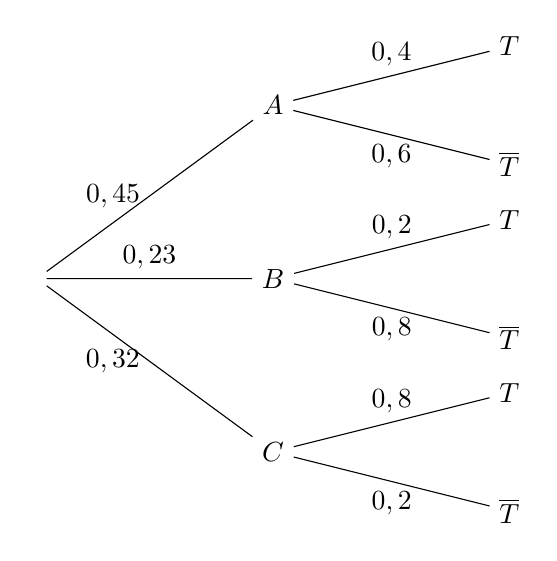
\begin{tikzpicture}
		[level 1/.style={level distance=3cm,
			sibling distance=2.2cm},
		level 2/.style={level distance=3cm,
			sibling distance=1.5cm},
		]
		\node {} [grow'=right]
		child {node {$A$}
			child {node {$T$}
				edge from parent node[above] {$0,4$}
			}
			child {node {$\overline T$}
				edge from parent node[below] {$0,6$}
			}
			edge from parent node[left] {$0,45$}}
		child {node {$B$}
			child {node {$T$}
				edge from parent node[above] {$0,2$}
			}
			child {node {$\overline T$}
				edge from parent node[below] {$0,8$}
			}
			edge from parent node[above] {$0,23$}}
		child {node {$C$}
			child {node {$T$}
				edge from parent node[above] {$0,8$}
			}
			child {node {$\overline T$}
				edge from parent node[below] {$0,2$}
			}	edge from parent node[left] {$0,32$}}
		
		;
	\end{tikzpicture}
\end{center}
	
	\subsection*{3.}
	
	Il faut trouver \(p(A \cap T) = p(A) \times p_A(T) = 0,45 \times 0,4 = 0,18\).
	
	\subsection*{4.}
	
	On a de même \(p(B \cap T) = p(B) \times p_B(T) = 0,23 \times 0,2 = 0,046\), puis
	\[
	p(C \cap T) = p(C) \times p_C(T) = 0,32 \times 0,8 = 0,256.
	\]
	
	D’après la loi des probabilités totales :
	\[
	p(T) = p(A \cap T) + p(B \cap T) + p(C \cap T) = 0,18 + 0,046 + 0,256 = 0,482.
	\]
	
	\subsection*{5.}
	
	Il faut trouver \(p_T(C) = \dfrac{p(T \cap C)}{p(T)} = \dfrac{p(C \cap T)}{p(T)} = \dfrac{0,256}{0,482} \approx 0,5311\), soit 0,531 au millième près.
	

	

	

